\section{Learnings and Conclusion} \label{section:luckypatcher-learnings}
%START TEXT INPUT
This is my real text! Rest might be copied or not be checked!
%START TEXT INPUT

%
first patching point could be the initial call, in case modified lvl patching initial call would be not enough since the on success block could contain important code (like ui creation) then it would be useless, target on specific points where decisions are made to alter as few code as possible

since automated customizations have to be implemented to trick it
make false checks to detect tampering -see- user patch

amazon/samsung not much to do since from company, beyond control of developer since injection after developer and a library provided by samsung which is only called, that is why the following not simple methods target lvl

known bytecode patterns, replace with custom, makes mechanism useless

following present ways of protecting against patching attempts, especially predefined recipes circumventing the LVL
high motivation, the patterns/patching modes cover many apps, more than custom

should not use one but many methods
solution for current version of lucky patcher, future might be different, arms race scenario
\cite{munteanLicense}
%

\begin{figure}[h]
    \centering
    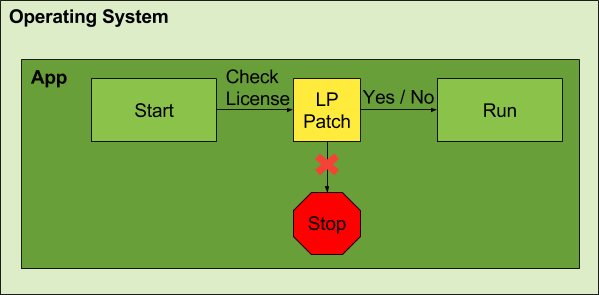
\includegraphics[width=0.8\textwidth]{data/verificationNowAttack.png}
    \caption{Abstraction of the current attack on the license verification mechanism}
    \label{fig:verificationNowAttack}
\end{figure}

nur ja/nein test bzw ergebnis zuweisung und drauf folgender test kann IMMER geskippt werden, vergleich figure~\ref{fig:verificationNow}



fügt keinen code hinzu sondern ersetzt commands => checksum/signature
